\subsect{Casos de uso}{casos_de_uso}

En un proyecto software, los casos de uso son una técnica para la captura de requisitos de un sistema~\cite{use_cases}.
Un caso de uso describe una unidad discreta de trabajo que puede ser realizada por el sistema, formada por un conjunto
de acciones que el sistema realiza.\ El siguiente diagrama representa los casos de uso básicos detectados para
la aplicación:

\begin{figure}[H]
	\centering
	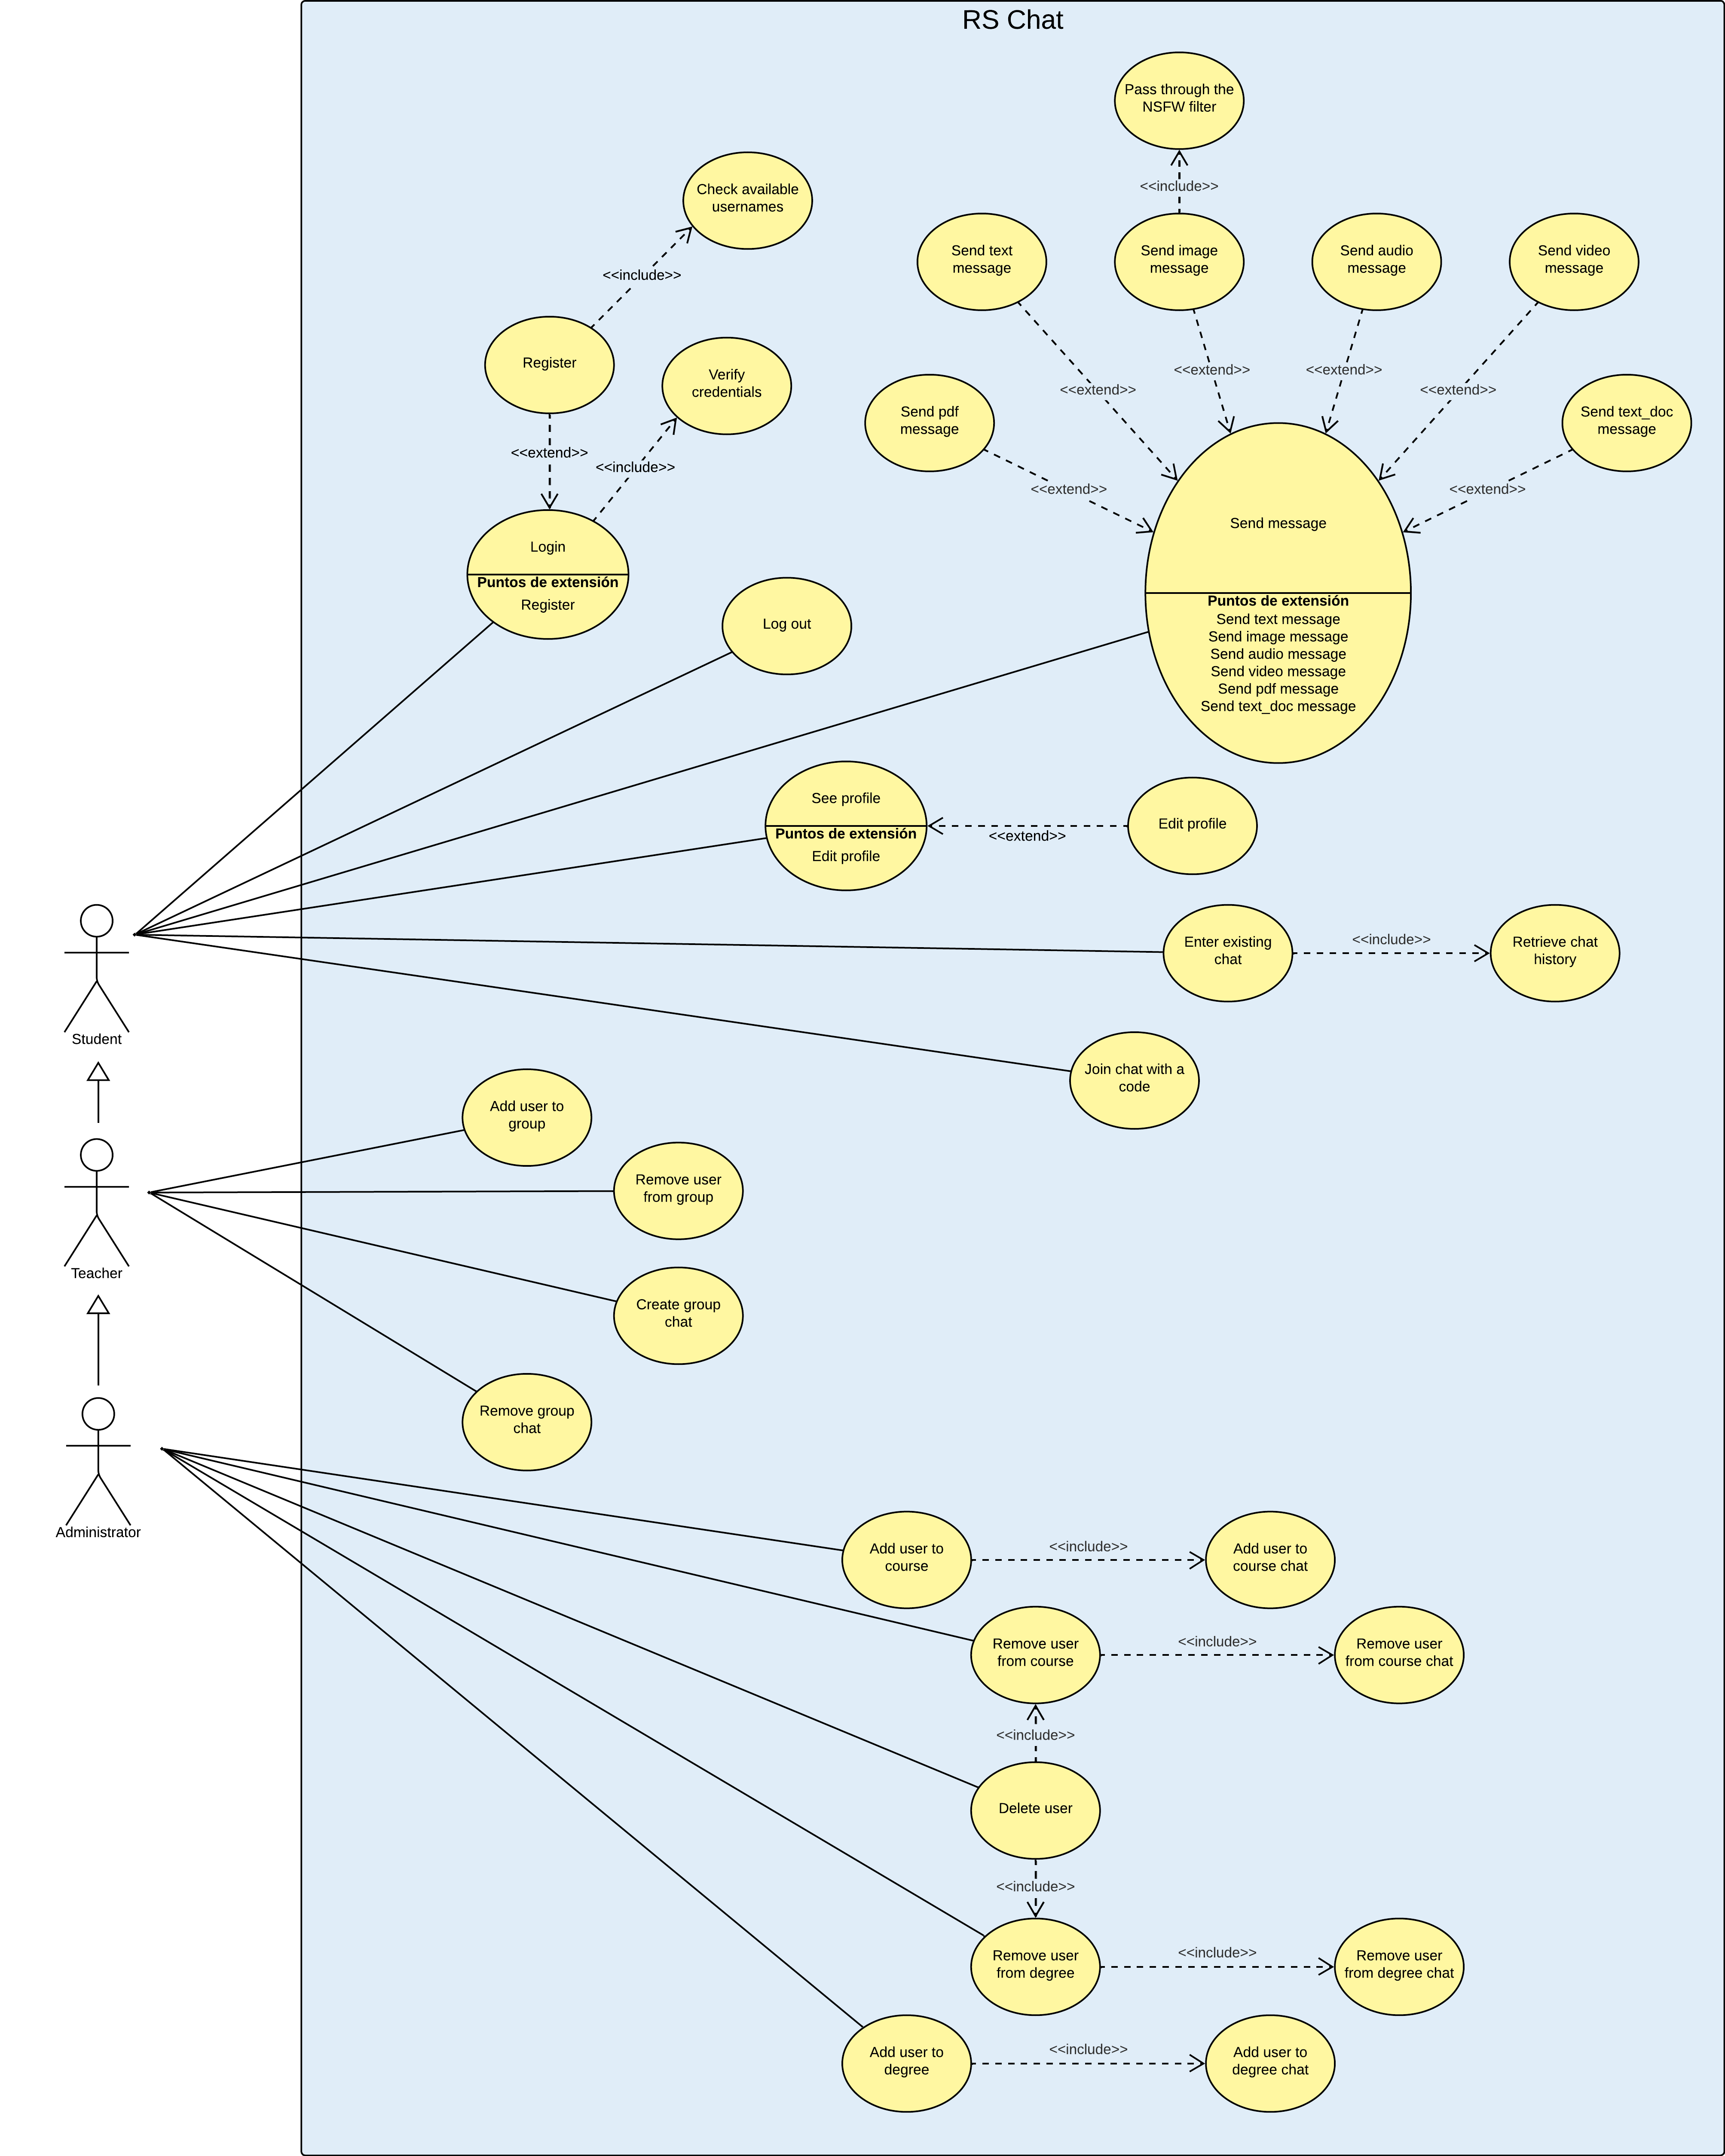
\includegraphics[width=0.8\textwidth]{res/images/RSChat-Diagrams-Usecases}
	\caption{Diagrama de casos de uso.}
	\label{fig:casosDeUso}
\end{figure}

En el diagrama se muestran los tres roles de usuarios que pueden existir en la aplicación (estudiante, profesor y
administrador).\ Debido a que existe \boldFont{herencia} de roles, los casos de uso que pertenecen a los estudiantes,
también pertenecen a los profesores y administradores, y los casos de uso de los profesores, también los
tienen los administradores.

\begin{itemize}
	\item Casos de uso de \underline{estudiantes}:
	\begin{itemize}
		\item \boldFont{Login}:
		Cuando un usuario inicia sesión, se realiza la verificación de sus credenciales (\textit{Verify credentials})
		para dar acceso a la aplicación.\ Como caso excepcional se encuentra el caso de que el usuario no esté
		registrado, en cuyo caso debe hacer el registro (\textit{Register}), que comprueba si hay usuarios con el mismo
		nombre de usuario (\textit{Check available usernames}).
		\item \boldFont{Log out}:
		El usuario puede cerrar sesión en cualquier momento.
		\item \boldFont{Send message}:
		Este caso de uso permite al usuario enviar un mensaje en un chat.\ Los puntos de extensión en este caso de uso
		representan el tipo de mensaje que se puede enviar (texto, imagen, vídeo, audio, etc.).
		Los mensajes que contengan imágenes se enviarán a un filtro NSFW para comprobar si son aptas para todos los
		públicos (\textit{Pass through the NSFW filter}).
		\item \boldFont{See profile}:
		El usuario puede ver su perfil, que contiene su información personal pudiendo editarlo (\textit{Edit profile}).
		\item \boldFont{Enter existing chat}:
		El usuario puede entrar en uno de los chats que se ofrezcan en la página principal de la aplicación.
		Al acceder a un chat, se cargan los mensajes que contiene (\textit{Retrieve chat history}).
		\item \boldFont{Join chat with a code}:
		Este caso de uso permite a un usuario unirse a un chat mediante un código que le proporciona el creador del
		mismo.
	\end{itemize}

	\item Casos de uso de \underline{profesores}:
	\begin{itemize}
		\item \boldFont{Add user to group}:
		Los profesores pueden añadir a un estudiante a un grupo de alumnos.
		\item \boldFont{Remove user from group}:
		Los profesores pueden eliminar a un estudiante de un grupo de alumnos.
		\item \boldFont{Create group chat}:
		Los profesores pueden crear un chat grupal para los alumnos de un grupo.
		\item \boldFont{Remove group chat}:
		Los profesores pueden eliminar un chat grupal.
	\end{itemize}

	\item Casos de uso de \underline{administradores}:
	\begin{itemize}
		\item \boldFont{Add user to course}:
		Los administradores tienen la capacidad de añadir a un usuario a un curso.\ Automáticamente, el usuario creado
		se añade al chat grupal del curso (\textit{Add user to course chat}).
		\item \boldFont{Add user to degree}:
		Igual que el anterior, pero añadiendo al usuario a un grado (\textit{Add user to degree chat}).
		\item \boldFont{Remove user from course}:
		Los administradores pueden eliminar a un usuario de un curso, y seguidamente ese usuario también se eliminará
		del chat grupal del curso.
		\item \boldFont{Remove user from degree}:
		Igual que el anterior, pero eliminando al usuario de un grado (\textit{Remove user from degree chat}).
		\item \boldFont{Delete user}:
		Los administradores pueden eliminar a un usuario de la aplicación.\ Al eliminarlo, se ejecutarán los casos de
		uso \textit{Remove user from course} y \textit{Remove user from degree}.
	\end{itemize}
\end{itemize}
